\documentclass{amsart}

\input{../preamble_general.tex}

\author{Jalen Chrysos}
\title{An Additional Planar Graph Problem}

\begin{document}
	\maketitle 
	
%	\noindent \textbf{Problem}: 
%	\begin{enumerate}[(a)]
%		\item Show that it is impossible to make a soccer ball using \textit{only} hexagonal patches, such that every vertex has degree exactly 3.
%		\item Now suppose that both hexagons and pentagons are permitted. Now it is possible to create a 3-regular ball. Show that the number of pentagons is fixed, and determine this number.\\
%	\end{enumerate}

%	\noindent \textbf{Problem}: Show that the following graph is not planar:
%	
%	\begin{figure}[h]
%		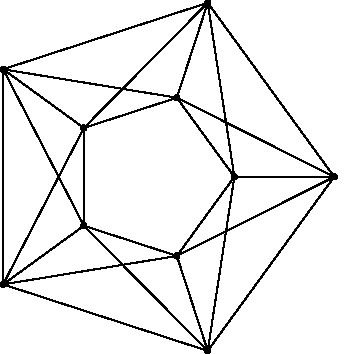
\includegraphics[width=0.3\textwidth]{./Asymptote_Figs/Planar1.pdf}
%	\end{figure}
%	
%	\noindent \textbf{Problem}: Show that the following graph is 3-colorable:
%	
%	\begin{figure}[h]
%		
%	\end{figure}
	
	\noindent \textbf{Problem 1}: Let $G$ be a plane graph with a Hamiltonian cycle. The cycle separates the plane into two regions, $A$ and $B$.\\
	
	\begin{minipage}{0.7\textwidth}
		\begin{enumerate}[(a)]
			\item (Grinberg's Theorem): For each face $F$ of $G$, let $\deg(F)$ denote the number of edges bounding $F$. Show that 
			$$
			\sum_{F\in A} \deg(F) - 2 = \sum_{F\in B} \deg(F) - 2
			$$
			(the first sum is over faces contained in region $A$, and the second is over faces in region $B$).
			\item Show that the plane graph pictured to the right has no Hamiltonian cycle.
		\end{enumerate}
	\end{minipage}
	\hspace{0.3cm}
	\begin{minipage}{0.3\textwidth}
		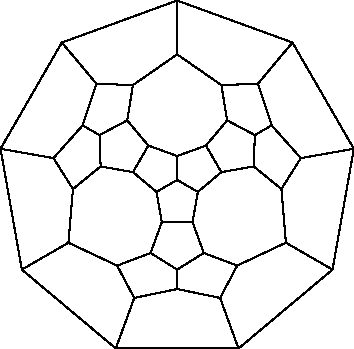
\includegraphics[width=0.8\textwidth]{./Asymptote_Figs/Grinberg3.pdf}
	\end{minipage}
	
	
	
\end{document}